%%
%%	Initial Management Report
%%	Created by Group02
%%
%%	10:27am 19/03/2013 
%%
%%	Use for SENG3011
%%

\documentclass[a4paper]{article}
\usepackage{a4wide}
\usepackage[normalem]{ulem} 
\usepackage{graphicx}
\usepackage{lscape}



\begin{document}

%%%%%%%%%%%%%%%%%%%%%%%%%%%%%%%%%%%%%%%%%%%%%%%%%%%%%%%
%%TITLE PAGE
\thispagestyle{empty}
\begin {center}
\Large\textbf{SENG3011} 

\Large\textbf{Intial Management Report}

\bigskip\Large\textbf{Group Number: 02}

\end{center}

\vspace*{16.5cm}
\begin{tabular}{|l|l|}
  \hline
  Version         & 1.0\\\hline
  Print Date      & 19/03/2013 10:26\\\hline
  Release Date    & dd/mm/yyyy\\\hline
  Release State   & Initial/Change/Final\\\hline
  Approval State  & Draft/Pending/Approved\\\hline
  Approved by     & \\\hline
  Prepared by     & \\\hline
  Reviewed by     & \\\hline
  Confidentiality Category  & Public/Confidential\\\hline
\end{tabular}
\pagebreak

%%%%%%%%%%%%%%%%%%%%%%%%%%%%%%%%%%%%%%%%%%%%%%%%%%%%%%%

%%%%%%%%%%%%%%%%%%%%%%%%%%%%%%%%%%%%%%%%%%%%%%%%%%%%%%%
%%REVISION CONTROL

\thispagestyle{plain}     % Turn on page numbering
\setcounter{page}{1}      % set page number counter
\renewcommand{\thepage}{\roman{page}}  % set page number to roman

\noindent{\Large\textbf{Document Revision Control}}\\[2ex]
\begin{tabular}{|l|l|l|l|}
  \hline
  Version & Date & Authors & Summary of Changes\\\hline\hline
	v1.0 & 20/03/2013 & Group02 & Added in Introduction           	\\\hline
	v1.1 & 12/09/2012 & Group02 &  		\\\hline
	v1.2 & 13/09/2012 & Group02 &   		\\\hline
	v1.3 & 13/09/2012 & Group02 &   		\\\hline
	v1.4 & 15/09/2012 & Group02 &  		\\\hline
	v1.5 & 15/09/2012 & Group02 & 		\\\hline
	v1.6 & 16/09/2012 & Group02 &  		\\\hline
	v1.7 & 15/09/2012 & Group02 &  		\\\hline
	v1.8 & 15/09/2012 & Group02 &   		\\\hline
\end{tabular}

\pagebreak

%%%%%%%%%%%%%%%%%%%%%%%%%%%%%%%%%%%%%%%%%%%%%%%%%%%%%%%

%%%%%%%%%%%%%%%%%%%%%%%%%%%%%%%%%%%%%%%%%%%%%%%%%%%%%%%
%%TABLE OF CONTENTS

\tableofcontents
\pagebreak
\listoffigures     %% delete if not required
\pagebreak         %% delete if there is no list of figures
\listoftables      %% delete if not required
\pagebreak         %% delete if there is no list of tables

%%%%%%%%%%%%%%%%%%%%%%%%%%%%%%%%%%%%%%%%%%%%%%%%%%%%%%%

%%%%%%%%%%%%%%%%%%%%%%%%%%%%%%%%%%%%%%%%%%%%%%%%%%%%%%%
%%MAIN

\setcounter{page}{1}     % Set page number counter
\renewcommand{\thepage}{\arabic{page}}  % print page number as arabic

\section {Introduction} 

This report is designed to discuss our initial prospects for the project and what we have in planned \\
for our final prototype. \\
\\ 
Within this report we will illustrate our Use Cases, Architecture and Sequence Diagrams,  \\
explain our chosen language and provide a project plan to which we hope to follow to   \\
complete our prototype.  \\
\\
We will be designing our report carefully following the Requirements List which has been \\
provided to us:  \\
\\
\indent\indent	1. Reading a correctly formatted Sirca orders file (1 day only) \\
\indent\indent 	2. Choosing an appropriate algorithmic trading strategy and setting its different \\
\indent\indent\indent	 		parameters \\
\indent\indent	3. Generating algorithmic orders for 1 particular day \\
\indent\indent	4. Evaluating algorithmic trades and providing feedback to the user \\
\indent\indent	5. Generating a strategy performance report \\ 
\indent\indent	6. GUI functions to control and use the Use Cases to load and execute orders \\ 
\indent\indent	7. GUI functions to visualise market data (spread, volume and depth) \\
\\
We will also aim to meet the Quality Requirements: \\
\\
\indent\indent	1. Speed of execution \\
\indent\indent 	2. Usability of the GUI \\
\indent\indent	3. Quality of the visualisation \\
\indent\indent	4. Quality of the strategic performance report \\	


\newpage	

\section {Use Cases}

From discussion between our members we were able to establish the following Use Cases: \\
\indent\indent	1. Placing a Bid Order	\\
\indent\indent	2. Placing an Ask Order 	\\	
\indent\indent	3. Amending a Bid Order 	\\
\indent\indent 	4. Amending an Ask Order \\	
\indent\indent	5. Deleting a Bid Order	\\
\indent\indent	6. Deleting an Ask Order 	\\ 
\\


\noindent{\bf Use Case 1}: Placing a bid Order \\
    \begin{tabular}{ | l | p{10cm} |}
    \hline
    	{\bf Actors} & Broker \\\hline
	{\bf Triggers} & The broker indicates they want to place a bid order. \\\hline
	{\bf Preconditions} & The broker has selected a price and quantity for the specific security. \\\hline
	{\bf Postconditions} & The order will be placed in the system. \\
	& The broker will have a Order ID for the bid. \\\hline
	{\bf Normal Flow} & Broker decides on a bid price and quantity for a specific security. \\
	& System accepts bid with bid price, appends to bid list and Order Book. \\
	& System returned generated order id to broker. \\\hline
    \end{tabular} \\\\

\noindent {\bf Use Case 2}: Placing an Ask Order \\ 
\begin{tabular}{ | l | p{10cm} |}\hline
	{\bf Actors} & Broker \\\hline
	{\bf Triggers} & The broker indicates they want to place an ask order.  \\\hline
	{\bf Preconditions} & The broker has selected a price and quantity for the specific security. \\\hline
	{\bf Postconditions} & The order will be placed in the system.  \\
	& The broker will have a Order ID for the ask order. \\\hline
	{\bf Normal Flow} & Broker decides on an ask price and quantity for a specific security. \\
	& System accepts with ask price, appends to ask list and Order Book. \\
	& System returned generated Order ID to broker. \\\hline
\end{tabular} \\\\

\noindent {\bf Use Case 3}: Amending a Bid Order \\ 
\begin{tabular}{ | l | p{10cm} |}\hline
	{\bf Actors} & Broker \\\hline
	{\bf Triggers} & The broker indicates they want to amend a bid order. \\\hline
	{\bf Preconditions} & The broker has indicated a change in the original price or quantity for the specific security. \\
	& The bid Order ID will already be in the system.  \\\hline
	{\bf Postconditions} & The broker will have a new Order ID for amended Order. \\\hline
	{\bf Normal Flow} & Broker decides on a change on price or quantity for original bid order. \\
	& System accepts the new price/quantity. \\
	& Cancels the old Order ID. \\
	& Creates a new Order ID. \\\hline
\end{tabular} \\\\

\noindent {\bf Use Case 4}: Amending an Ask Order \\ 
\begin{tabular}{ | l | p{10cm} |}\hline
	{\bf Actors} & Broker \\\hline
	{\bf Triggers} & The broker wants to change the price or amount of their existing ask order.  \\\hline
	{\bf Preconditions} & The broker has an existing ask Order. \\
	& The broker wants to change the ask price or ask amount. \\\hline
	{\bf Postconditions} & The previous Order gets deleted. \\
	& A new order is created with the new ask price and amount. \\\hline
	{\bf Normal Flow} & The broker wants to update an existing order so the previous order is deleted and an new order is created. This prevents cheating as orders are prioritised by time, and a broker can take advantage of their placement in the queue to match a sell order. \\\hline
\end{tabular} \\\\

\noindent {\bf Use Case 5}: Deleting a Bid Order \\ 
\begin{tabular}{ | l | p{10cm} |}\hline
	{\bf Actors} & Broker \\\hline
	{\bf Triggers} & The broker indicates they want to remove a bid order. \\\hline
	{\bf Preconditions} & The broker has an existing bid in the system. The broker knows the Order ID. \\\hline
	{\bf Postconditions} & The Order will be removed from the system. \\\hline
	{\bf Normal Flow} & Broker decides to remove their bid order from the system. \\
	& System accepts the Order ID to remove. \\
	& Bid list and order book are updated.  \\\hline
\end{tabular} \\\\

\noindent {\bf Use Case 6}: Deleting an Ask Order \\ 
\begin{tabular}{ | l | p{10cm} |}\hline
	{\bf Actors} & Broker \\\hline
	{\bf Triggers} & The broker indicates they want to remove an ask order. \\\hline
	{\bf Preconditions} & The broker has an existing ask in the system. The broker knows the Order ID. \\\hline
	{\bf Postconditions} & The Order will be removed from the system.  \\\hline
	{\bf Normal Flow} & Broker decides to remove their ask order from the system. \\
	& System accepts the Order ID to remove. \\
	& Ask list and order book are updated. \\\hline
\end{tabular} \\\\

\begin {landscape}
\section {Architecture Diagram}
\begin{figure}
  \caption{Architectural Diagram.}
  \centering
    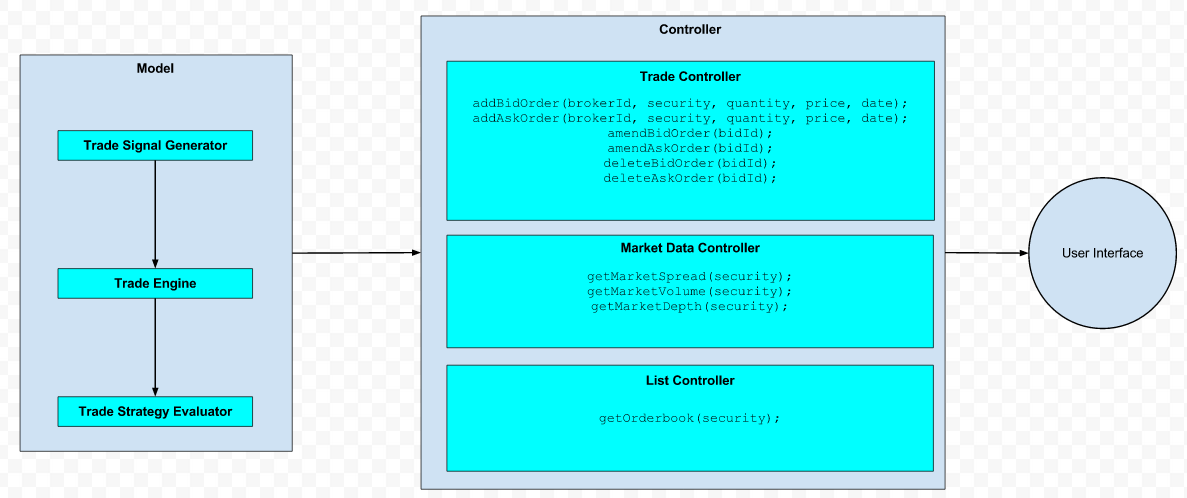
\includegraphics[width=1.6\textwidth]{images/ADiagram}
\end{figure}
\end {landscape}

\section {Sequence Diagram} 

\begin{figure}[h]
  \caption{Use Case 1: addBidOrder}
  \centering
    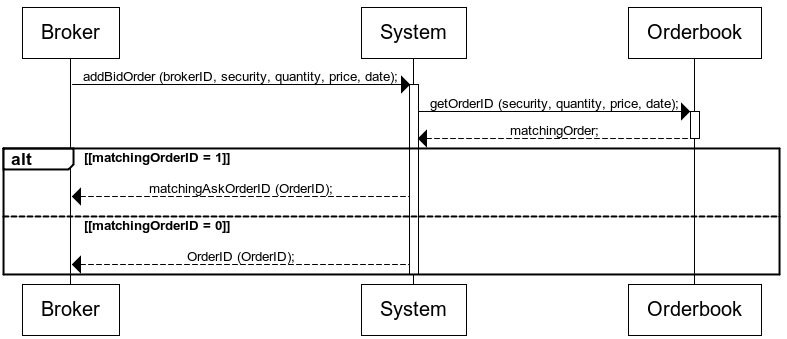
\includegraphics[width=1\textwidth]{images/addBidOrder}
\end{figure}

\begin{figure}[h]
  \caption{Use Case 2: addAskOrder}
  \centering
    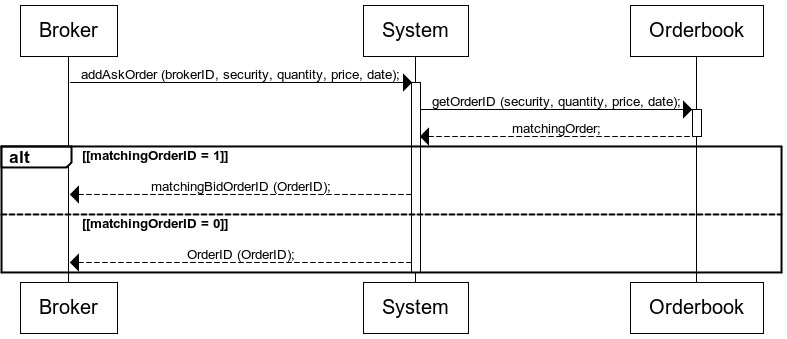
\includegraphics[width=1\textwidth]{images/addAskOrder}
\end{figure}

\newpage

\begin{figure}
  \caption{Use Case 3: amendBidOrder}
  \centering
    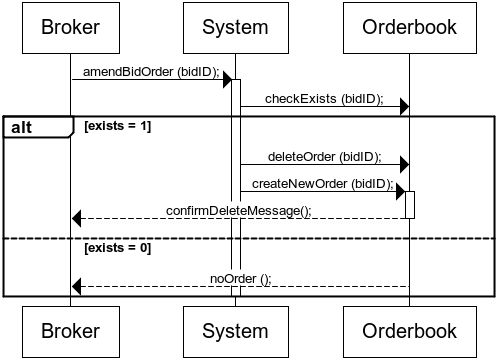
\includegraphics[width=1\textwidth]{images/amendBidOrder}
\end{figure}

\newpage

\begin{figure}[h]
  \caption{Use Case 4: amendAskOrder}
  \centering
    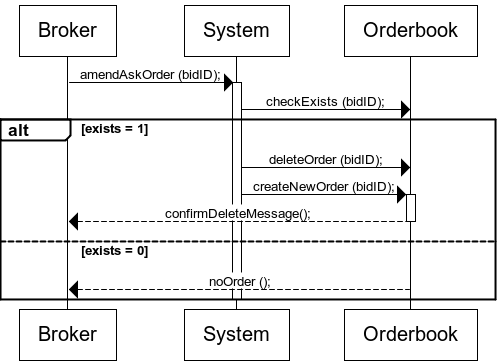
\includegraphics[width=1\textwidth]{images/amendAskOrder}
\end{figure}

\begin{figure}
  \caption{Use Case 5: deleteBidOrder}
  \centering
    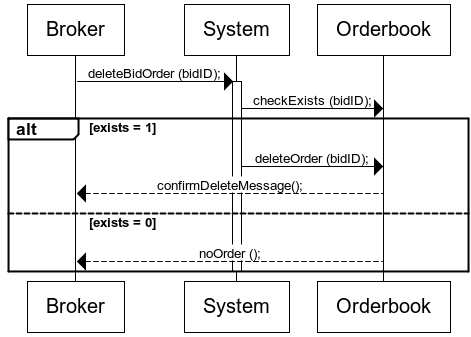
\includegraphics[width=1\textwidth]{images/deleteBidOrder}
\end{figure}

\begin{figure}
  \caption{Use Case 6: deleteAskOrder}
  \centering
    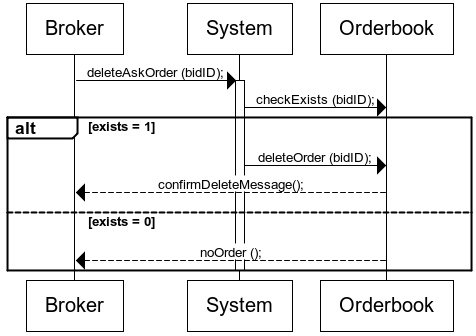
\includegraphics[width=1\textwidth]{images/deleteAskOrder}
\end{figure}




\section{LOLZ}
























\end {document}